\documentclass[10pt,UTF8]{beamer}
\usepackage[absolute,overlay]{textpos}
\usepackage{advdate}
\usepackage{mathrsfs}
\newcommand{\yesterday}{{\AdvanceDate[-1]\today}}
\newcommand{\tomorrow}{{\AdvanceDate[1]\today}}

\usetheme{metropolis}
\usepackage{appendixnumberbeamer}
\usepackage{bm}
\usepackage{mathbbol}
\usepackage{amsmath,amssymb,amsfonts,bbm}
\usepackage{booktabs}
\usepackage{graphics}
\usepackage{graphicx}
\usepackage{xcolor}
\usepackage[export]{adjustbox}
\usepackage{float}
\usepackage[scale=2]{ccicons}
\usepackage{pgfplots}
\usepackage{tikz}
\usepgfplotslibrary{dateplot}
\usetikzlibrary{calc}
\setbeamercolor{block title}{use=normal text, fg=normal text.fg,bg=normal text.bg!80!fg}
\setbeamercolor{mymath}{use={block title, normal text}, bg=block title.bg!50!normal text.bg}
\setbeamercolor{mymath2}{bg=blue!10, fg=black}
\usepackage{xspace}
\newcommand{\themename}{\textbf{\textsc{metropolis}}\xspace}
\graphicspath{{./}{../figures/}{../figures/2Dphi4/}{../figures/3Dphi4/}{../figures/2Dphi4/correlation_k=0.26/}{../figures/2Dphi4/correlation_k=0.2705/}{../figures/2Dphi4/correlation_k=0.28/}}

\title{Score-Based Diffusion Models for\\[4pt] 2D and 3D $\phi^4$ Lattice Field Theory}
\date{\today}
\author{Yang-yang Tan}

\definecolor{burgundy}{RGB}{127, 0, 32}
\definecolor{Kleinblue}{RGB}{0, 47, 167}

\begin{document}
\maketitle

{
\metroset{sectionpage=none}
\section{Outline}
}
\metroset{sectionpage=progressbar}

\begin{frame}{Outline}
\tableofcontents
\end{frame}

%======================================================================
\section{Critical Points from Wolff + FA-HMC}
%======================================================================

\begin{frame}{Lattice $\phi^4$ Action}
The scalar $\phi^4$ theory on a $D$-dimensional $L^D$ lattice with periodic BC:
\begin{equation}
    S[\phi] = \sum_{x} \Bigl[
      -2\kappa \sum_{\mu=1}^{D} \phi_x\,\phi_{x+\hat\mu}
      + \phi_x^2 + \lambda\bigl(\phi_x^2 - 1\bigr)^2
    \Bigr]
\end{equation}

\begin{itemize}
    \item $\kappa$: hopping parameter, \quad $\lambda$: quartic self-coupling
    \item $\mathbb{Z}_2$-breaking phase transition at $\kappa_c(\lambda)$
    \item \textbf{2D}: $\lambda=0.022$, \quad \textbf{3D}: $\lambda=0.9$
\end{itemize}

\vspace{0.3cm}
\textbf{Sampling algorithm:} Wolff cluster flips + Fourier-accelerated HMC
\begin{itemize}
    \item FA-HMC: momentum-dependent mass $M(\hat p) = \hat p^2 + m_\text{eff}^2$ via FFT
    \item Wolff cluster: flips $\phi_x \to -\phi_x$ to decorrelate magnetisation
\end{itemize}
\end{frame}

\begin{frame}{2D: Order Parameter and Susceptibility}
\begin{columns}[T]
\begin{column}{0.5\textwidth}
    \begin{figure}
        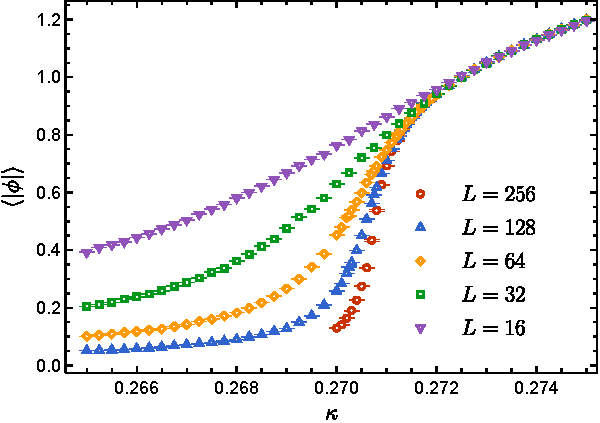
\includegraphics[width=\textwidth]{orderparameter_2d_wolff_fahmc.pdf}
    \end{figure}
    \vspace{-0.3cm}
    {\small Order parameter $\langle|\bar\phi|\rangle$ vs.\ $\kappa$ for $L=16$--$256$.
    Transition sharpens with $L$.}
\end{column}
\begin{column}{0.5\textwidth}
    \begin{figure}
        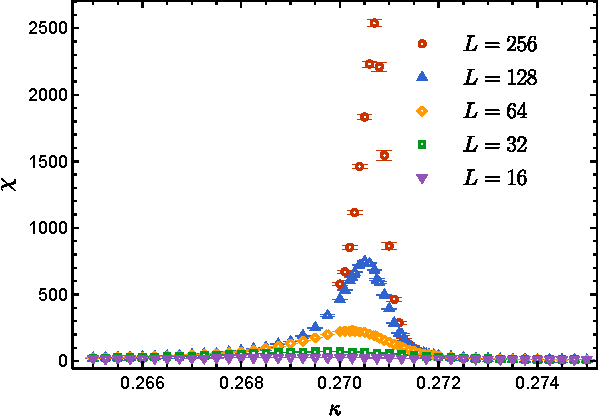
\includegraphics[width=\textwidth]{chi_2d_wolff_fahmc_1.pdf}
    \end{figure}
    \vspace{-0.3cm}
    {\small Susceptibility $\chi$ vs.\ $\kappa$. Peak grows $\sim L^{\gamma/\nu}$ ($\gamma/\nu=7/4$, 2D Ising).}
\end{column}
\end{columns}
\end{frame}

\begin{frame}{2D: Susceptibility and Binder Cumulant}
\begin{columns}[T]
\begin{column}{0.5\textwidth}
    \begin{figure}
        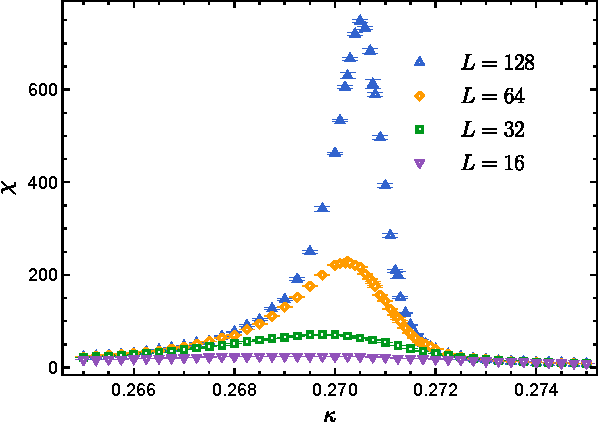
\includegraphics[width=\textwidth]{chi_2d_wolff_fahmc_2.pdf}
    \end{figure}
    \vspace{-0.3cm}
    {\small Susceptibility $\chi$ (alternative representation).}
\end{column}
\begin{column}{0.5\textwidth}
    \begin{figure}
        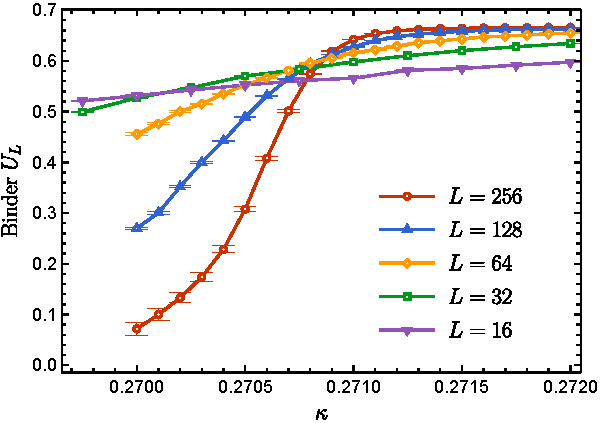
\includegraphics[width=\textwidth]{binder_2d_wolff_fahmc.pdf}
    \end{figure}
    \vspace{-0.3cm}
    {\small Binder cumulant $U_L$ vs.\ $\kappa$ for $L=16$--$256$.
    Curves cross at $\kappa_c$.}
\end{column}
\end{columns}
\end{frame}

\begin{frame}{2D Critical Point: $\kappa_c \approx 0.27088$}
\begin{columns}[T]
\begin{column}{0.5\textwidth}
    \begin{figure}
        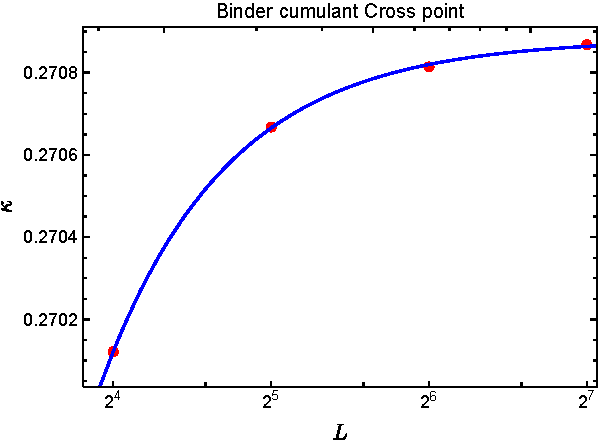
\includegraphics[width=\textwidth]{bindercross_2d_wolff_fahmc.pdf}
    \end{figure}
    \vspace{-0.3cm}
    {\small Binder crossing analysis $\Rightarrow$ $\kappa_c({\lambda=0.022}) \approx 0.27088$.}
\end{column}
\begin{column}{0.5\textwidth}
    \vspace{1cm}
    \begin{itemize}
        \item 2D Ising universality class
        \item $\lambda = 0.022$
        \item Three $\kappa$ values for DM study:
        \begin{itemize}
            \item $0.26$ (symmetric)
            \item $0.2705 \approx \kappa_c$ (critical)
            \item $0.28$ (broken)
        \end{itemize}
    \end{itemize}
\end{column}
\end{columns}
\end{frame}

\begin{frame}{3D: Order Parameter and Susceptibility}
\begin{columns}[T]
\begin{column}{0.5\textwidth}
    \begin{figure}
        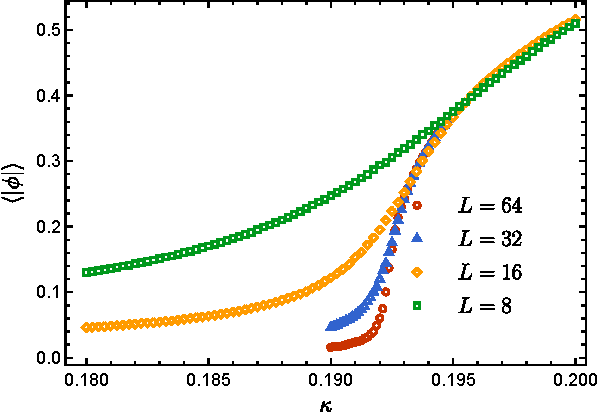
\includegraphics[width=\textwidth]{orderparameter_3d_wolff_fahmc.pdf}
    \end{figure}
    \vspace{-0.3cm}
    {\small Order parameter $\langle|\bar\phi|\rangle$ vs.\ $\kappa$ for $L=8$--$64$.}
\end{column}
\begin{column}{0.5\textwidth}
    \begin{figure}
        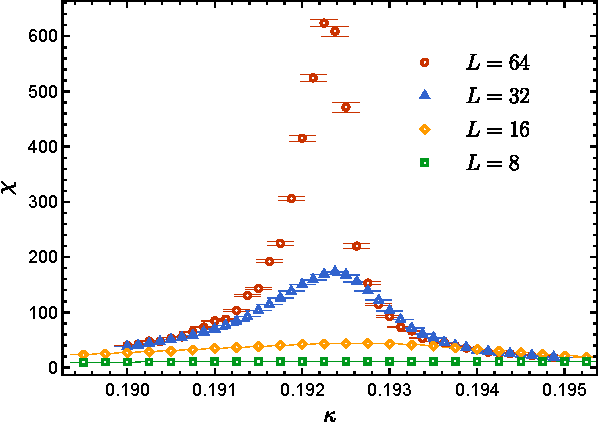
\includegraphics[width=\textwidth]{chi_3d_wolff_fahmc.pdf}
    \end{figure}
    \vspace{-0.3cm}
    {\small Susceptibility $\chi$ vs.\ $\kappa$. Peak converges toward $\kappa_c$.}
\end{column}
\end{columns}
\end{frame}

\begin{frame}{3D Critical Point: $\kappa_c \approx 0.19225$}
\begin{columns}[T]
\begin{column}{0.5\textwidth}
    \begin{figure}
        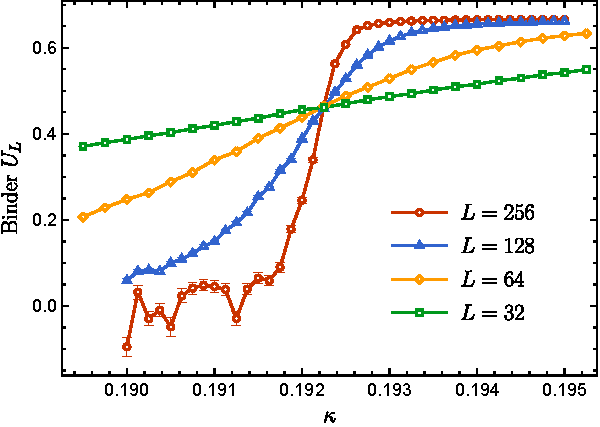
\includegraphics[width=\textwidth]{binder_3d_wolff_fahmc.pdf}
    \end{figure}
    \vspace{-0.3cm}
    {\small Binder cumulant crossing $\Rightarrow$ $\kappa_c({\lambda=0.9}) \approx 0.19225$.}
\end{column}
\begin{column}{0.5\textwidth}
    \vspace{1cm}
    \begin{itemize}
        \item 3D Ising universality class ($\nu \approx 0.63$)
        \item $\lambda = 0.9$
        \item Three $\kappa$ values for DM study:
        \begin{itemize}
            \item $0.18$ (symmetric)
            \item $0.1923 \approx \kappa_c$ (critical)
            \item $0.2$ (broken)
        \end{itemize}
    \end{itemize}
\end{column}
\end{columns}
\end{frame}

%======================================================================
\section{Score-Based Diffusion Model}
%======================================================================

\begin{frame}{Score-Based Generative Model: Setup}
\textbf{Forward SDE} (Variance-Exploding):
\begin{equation}
    \mathrm{d}\phi = \sigma^t\,\mathrm{d}W, \quad \sigma(t) = \sqrt{(\sigma^{2t}-1)/2\log\sigma}
\end{equation}

\textbf{Reverse SDE} (sampling):
\begin{equation}
    \mathrm{d}\phi = -g^2(t)\,\nabla_\phi \log p_t(\phi)\,\mathrm{d}t + g(t)\,\mathrm{d}\bar{W}
\end{equation}

\textbf{Score matching loss}:
\begin{equation}
    \mathcal{L} = \mathbb{E}_{t,\phi_0,z}\!\left[\bigl\|s_\theta(\phi_0+\sigma(t)z,\,t)\cdot\sigma(t) + z\bigr\|^2\right]
\end{equation}

\begin{itemize}
    \item Train $s_\theta(\phi, t) \approx \nabla_\phi \log p_t(\phi)$
    \item Sample via Euler--Maruyama reverse integration
    \item Data normalised to $[-1,1]$ using global min/max
\end{itemize}
\end{frame}

\begin{frame}{NCSN++ Architecture}
\begin{figure}
    
\includegraphics[width=\textwidth]{architecture_ncsnpp.pdf}
\end{figure}
\vspace{-0.3cm}
\begin{itemize}
    \item \textbf{Circular padding} on all convolutions $\Rightarrow$ periodic BC
    \item Time $t$ encoded via Gaussian Fourier Projection (GFP) + MLP, additive
    \item 2D: \texttt{Conv2d} ($L=128$); \quad 3D: \texttt{Conv3d} ($L=64$)
    \item ResBlock: no residual connection (removed for training stability)
\end{itemize}
\end{frame}

%======================================================================
\section{Training Diagnostics}
%======================================================================

\begin{frame}{MALA Acceptance Rate as Diagnostic}
MALA proposal using the score network:
\begin{equation}
    \psi = \phi + h\,s_\theta(\phi, t_\text{mh}) + \sqrt{2h}\,\eta, \quad \eta \sim \mathcal{N}(0, \mathbbm{1})
\end{equation}
Accept/reject with exact action $e^{-S(\phi)}$:
\begin{equation}
    \alpha = \min\!\left\{1,\;\frac{e^{-S(\psi)}\,q(\phi|\psi)}{e^{-S(\phi)}\,q(\psi|\phi)}\right\}
\end{equation}

\begin{itemize}
    \item A well-trained score $\Rightarrow$ high acceptance rate
    \item Step size: $h = c/L^D$ \quad ($c=0.2$ universal across $D$)
    \item Evaluation time: $t_\text{mh} = 10^{-4}$ \quad (maximises diagnostic power)
    \item $N=1024$ (2D) or $N=256$ (3D) reference configs, single MH step
\end{itemize}
\end{frame}

\begin{frame}{2D: Step-Size and $t_\text{mh}$ Calibration}
\begin{columns}[T]
\begin{column}{0.5\textwidth}
    \begin{figure}
        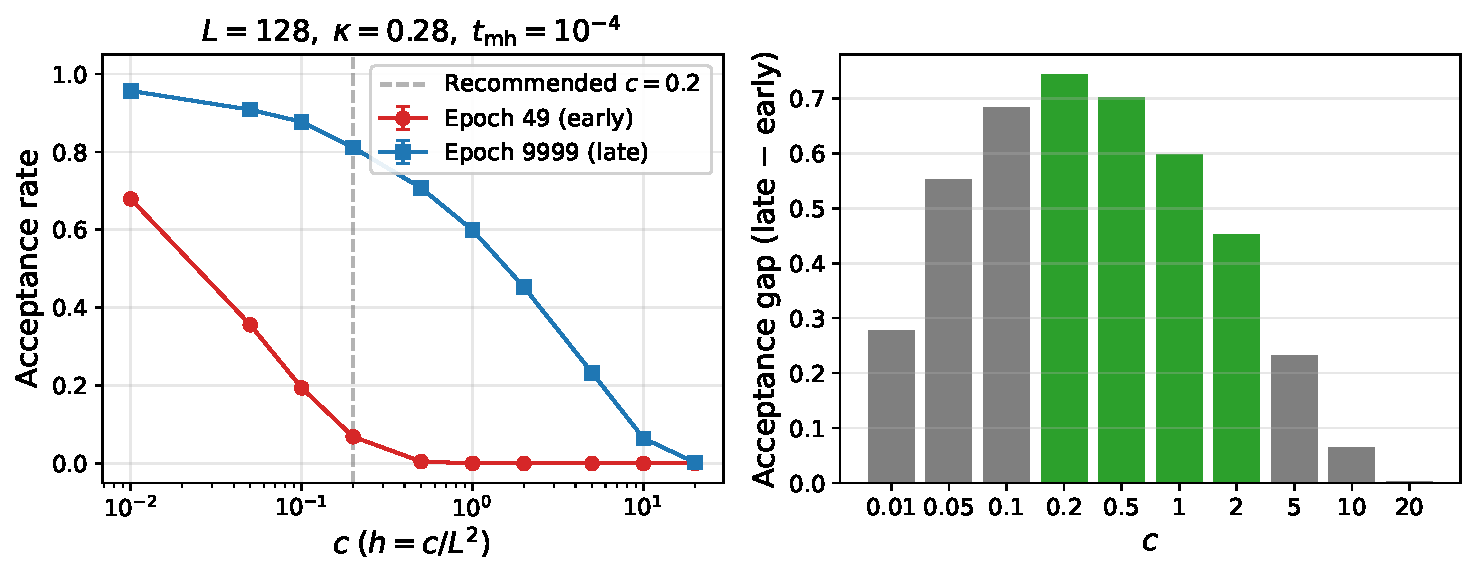
\includegraphics[width=\textwidth]{calibrate_h_L128_k0.28.pdf}
    \end{figure}
    \vspace{-0.3cm}
    {\small $h=c/L^2$: optimal $c=0.2$ at $L=128$.}
\end{column}
\begin{column}{0.5\textwidth}
    \begin{figure}
        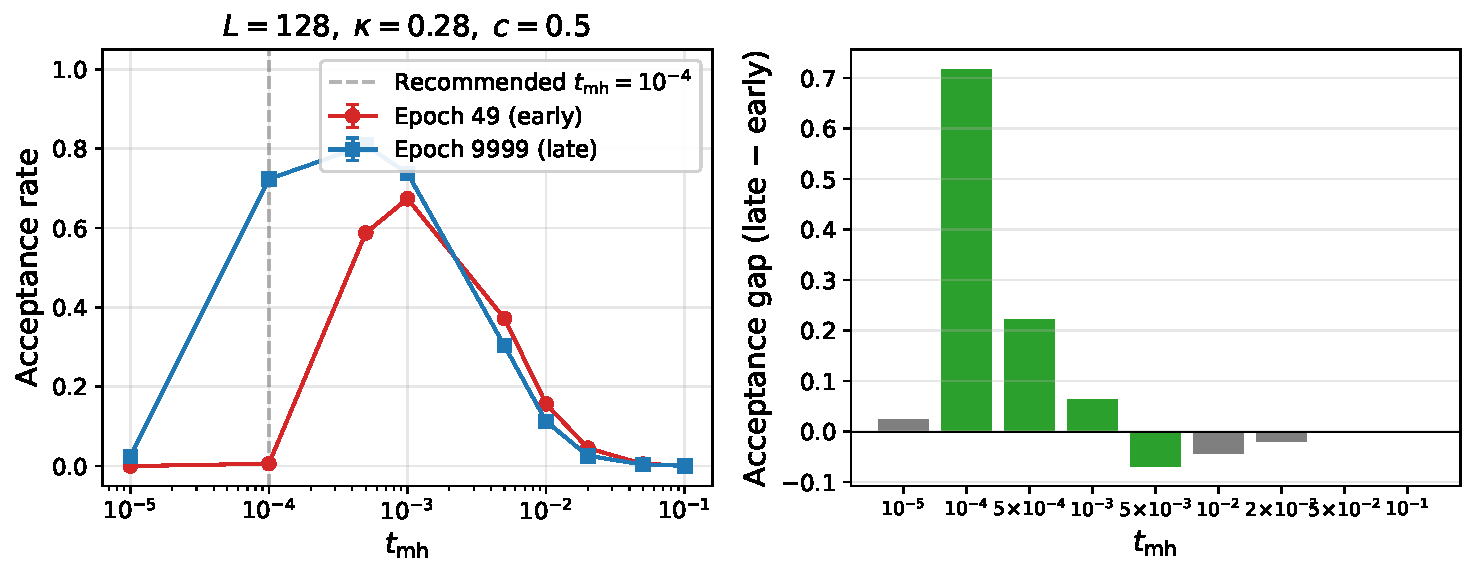
\includegraphics[width=\textwidth]{calibrate_t_mh_L128_k0.28.pdf}
    \end{figure}
    \vspace{-0.3cm}
    {\small $t_\text{mh}=10^{-4}$ maximises diagnostic power.\\
    Gap reverses for $t_\text{mh}\gtrsim 5\times10^{-3}$.}
\end{column}
\end{columns}
\end{frame}

\begin{frame}{2D: Acceptance Rate vs.\ Training Epoch}
\begin{columns}[T]
\begin{column}{0.55\textwidth}
    \begin{figure}
        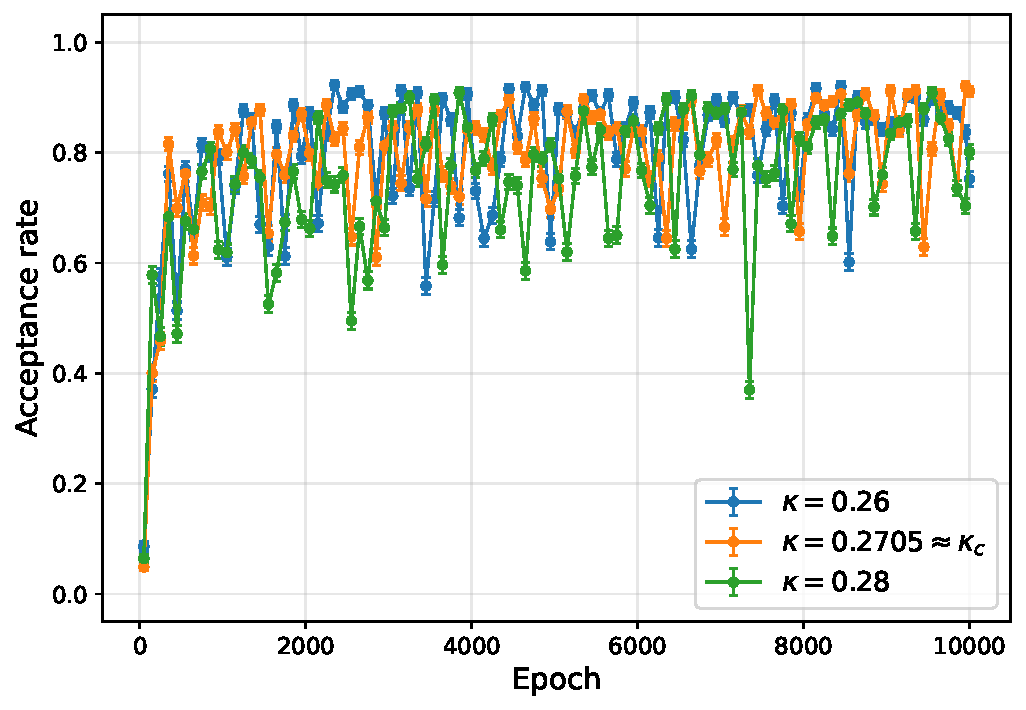
\includegraphics[width=\textwidth]{acceptance_vs_epoch_L128_combined.pdf}
    \end{figure}
    \vspace{-0.3cm}
    {\small $L=128$, three $\kappa$ values. Rises from $\sim 0$ to $60$--$90\%$.}
\end{column}
\begin{column}{0.45\textwidth}
    {\small
    \textbf{Late training} (ep.\ 3999--4999):
    \vspace{0.2cm}

    \begin{tabular}{ccc}
    \toprule
    $L$ & $\kappa\!=\!0.26$ & $0.28$ \\
    \midrule
    8   & $0.64$ & $0.63$ \\
    32  & $0.68$ & $0.68$ \\
    64  & $0.83$ & $0.75$ \\
    128 & $0.79$ & $0.75$ \\
    \bottomrule
    \end{tabular}

    \vspace{0.3cm}
    Acceptance rate increases with $L$ (conservative $h=c/L^2$ scaling).
    }
\end{column}
\end{columns}
\end{frame}

\begin{frame}{2D: Direct Score Quality}
\begin{figure}
    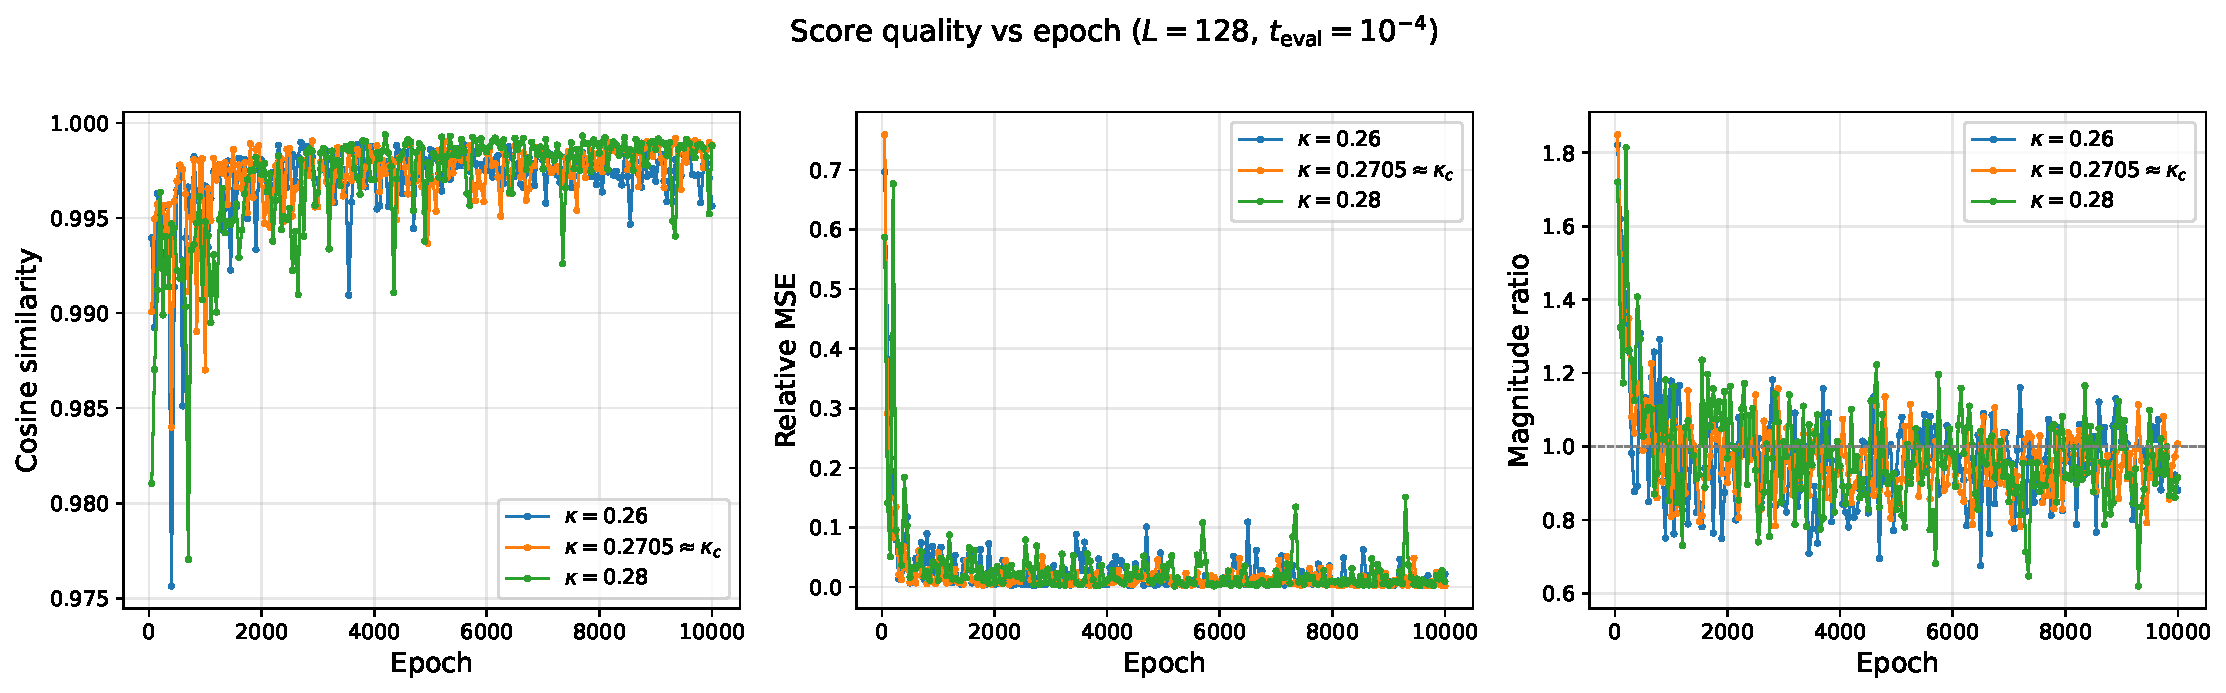
\includegraphics[width=\textwidth]{score_quality_vs_epoch_L128_3panel.pdf}
\end{figure}
\vspace{-0.3cm}
Compare $s_\theta(\phi, t)$ vs.\ $-\nabla_\phi S$ at $t_\text{eval}=10^{-4}$:
\begin{itemize}
    \item Cosine similarity: $0.99 \to 0.998$
    \item Relative MSE: drops $>10\times$
    \item Magnitude ratio: $\sim1.5 \to \sim 0.95$ (converges to 1)
\end{itemize}
\end{frame}

%======================================================================
\section{2D Propagator Results}
%======================================================================

\begin{frame}{2D Propagator: $\kappa=0.26$ (Symmetric Phase)}
\begin{figure}
    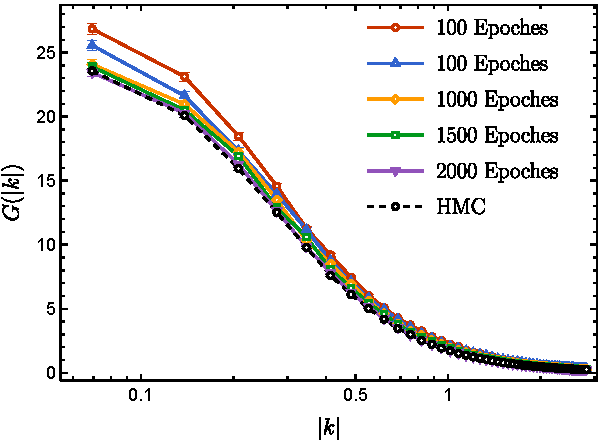
\includegraphics[width=0.5\textwidth]{prop_k=0.26_log.pdf}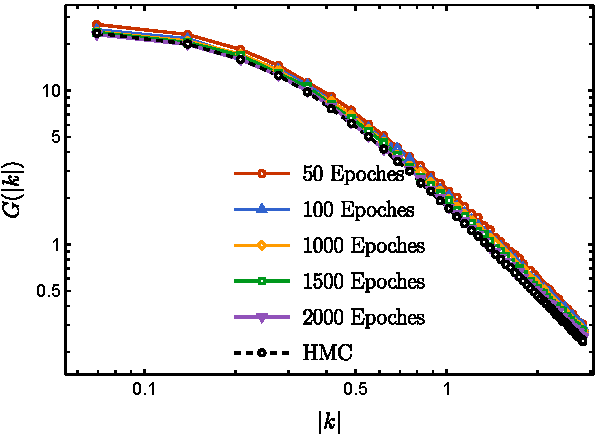
\includegraphics[width=0.5\textwidth]{prop_k=0.26_log_log.pdf}
\end{figure}
\vspace{-0.3cm}
$L=128$, $\lambda=0.022$. DM converges to HMC propagator with training.
\end{frame}

\begin{frame}{2D Propagator: $\kappa=0.2705$ (Near-Critical)}
\begin{figure}
    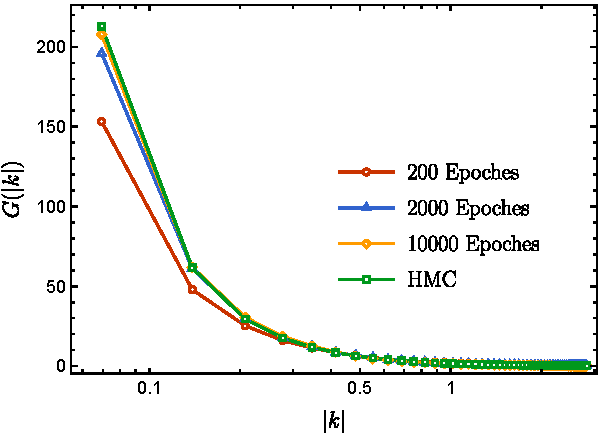
\includegraphics[width=0.5\textwidth]{prop_k=0.2705_log.pdf}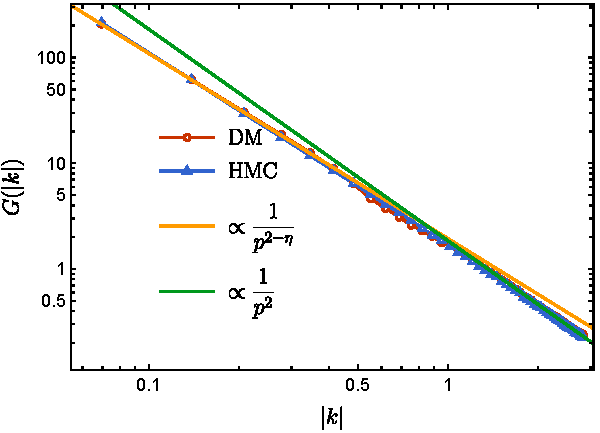
\includegraphics[width=0.5\textwidth]{prop_k=0.2705_log_log.pdf}
\end{figure}
\vspace{-0.3cm}
Most demanding: $\xi \to \infty$, power-law tail $G(p) \sim p^{-(2-\eta)}$. DM captures the IR behaviour.
\end{frame}

\begin{frame}{2D Propagator: $\kappa=0.28$ (Broken Phase)}
\begin{figure}
    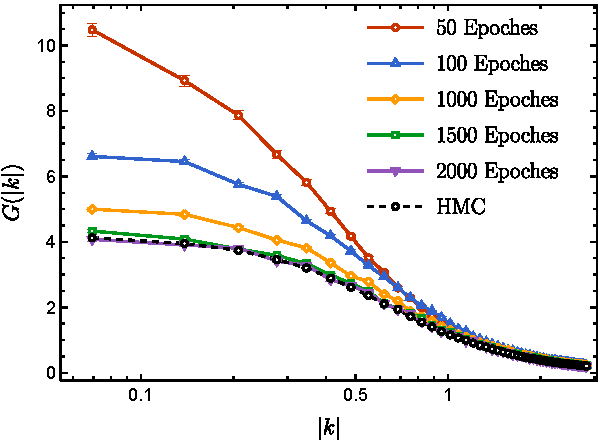
\includegraphics[width=0.5\textwidth]{prop_k=0.28_log.pdf}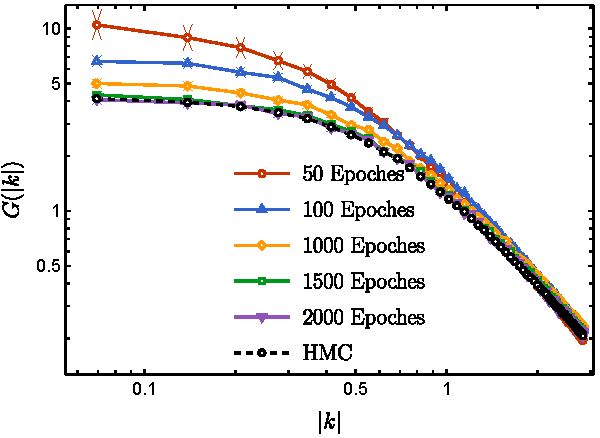
\includegraphics[width=0.5\textwidth]{prop_k=0.28_log_log.pdf}
\end{figure}
\vspace{-0.3cm}
Ordered phase with mass gap. Faithful reproduction by DM.
\end{frame}

%======================================================================
\section{3D Results}
%======================================================================

\begin{frame}{3D Training Loss Decomposition}
\begin{figure}
    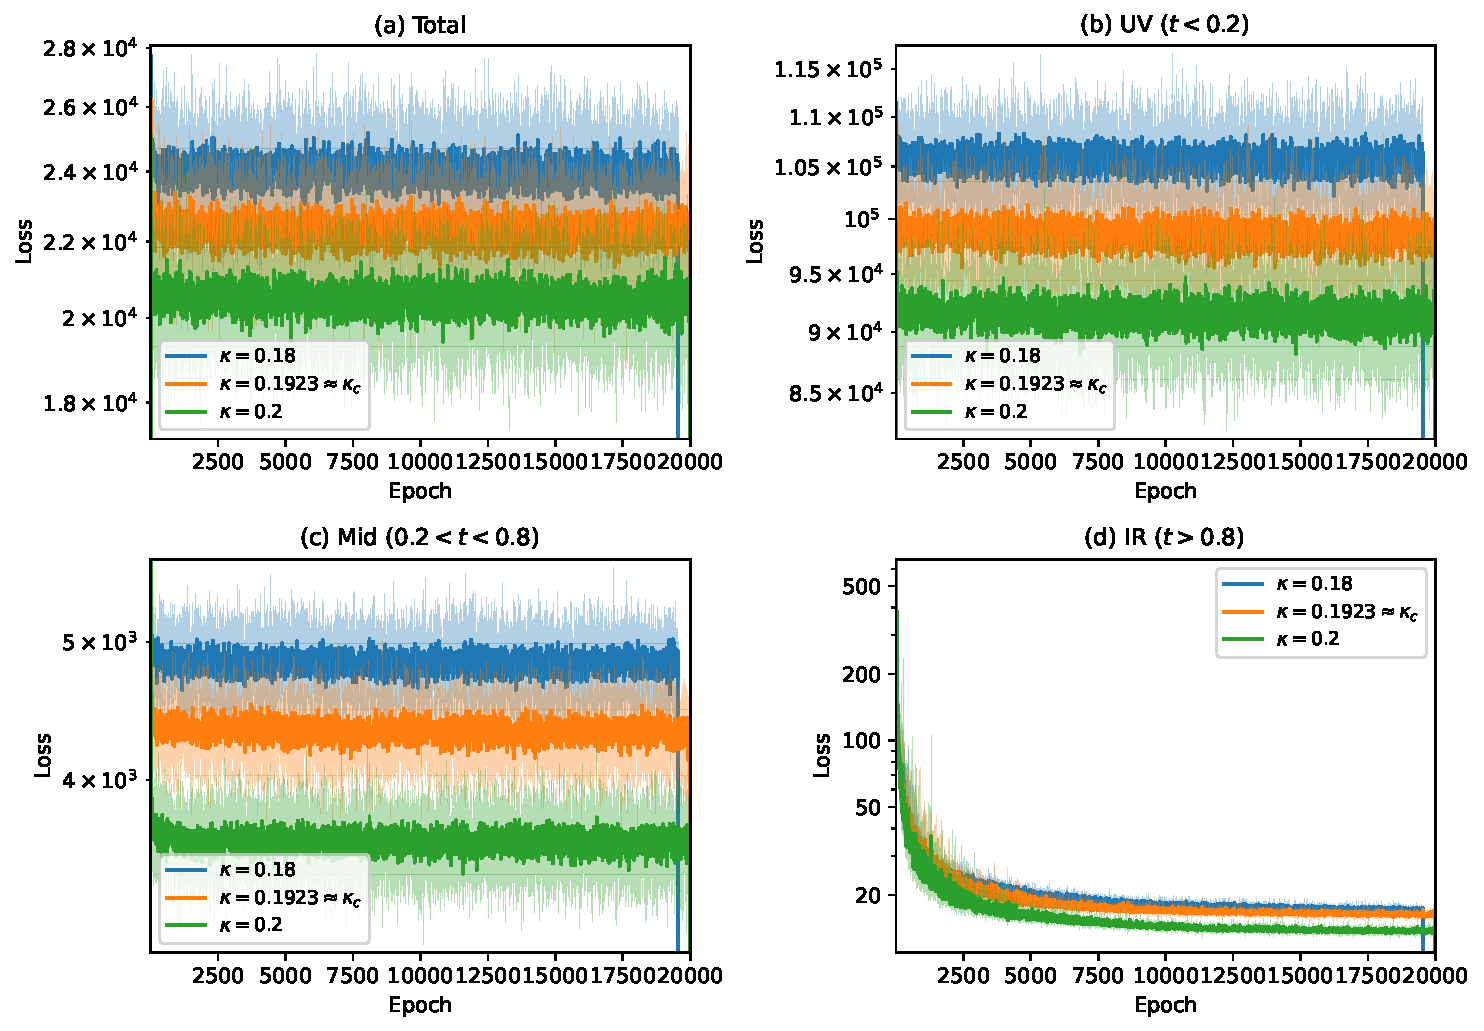
\includegraphics[width=\textwidth]{loss_3d_L64_decomposed.pdf}
\end{figure}
\vspace{-0.3cm}
$L=64$, $\lambda=0.9$. Loss decomposed by diffusion time $t$:
\begin{itemize}
    \item \textbf{UV} ($t<0.2$): short-distance modes
    \item \textbf{Mid} ($0.2<t<0.8$): intermediate
    \item \textbf{IR} ($t>0.8$): long-distance modes --- dominant, most $\kappa$-sensitive
\end{itemize}
\end{frame}

\begin{frame}{3D: Acceptance Rate Calibration}
\begin{columns}[T]
\begin{column}{0.5\textwidth}
    \begin{figure}
        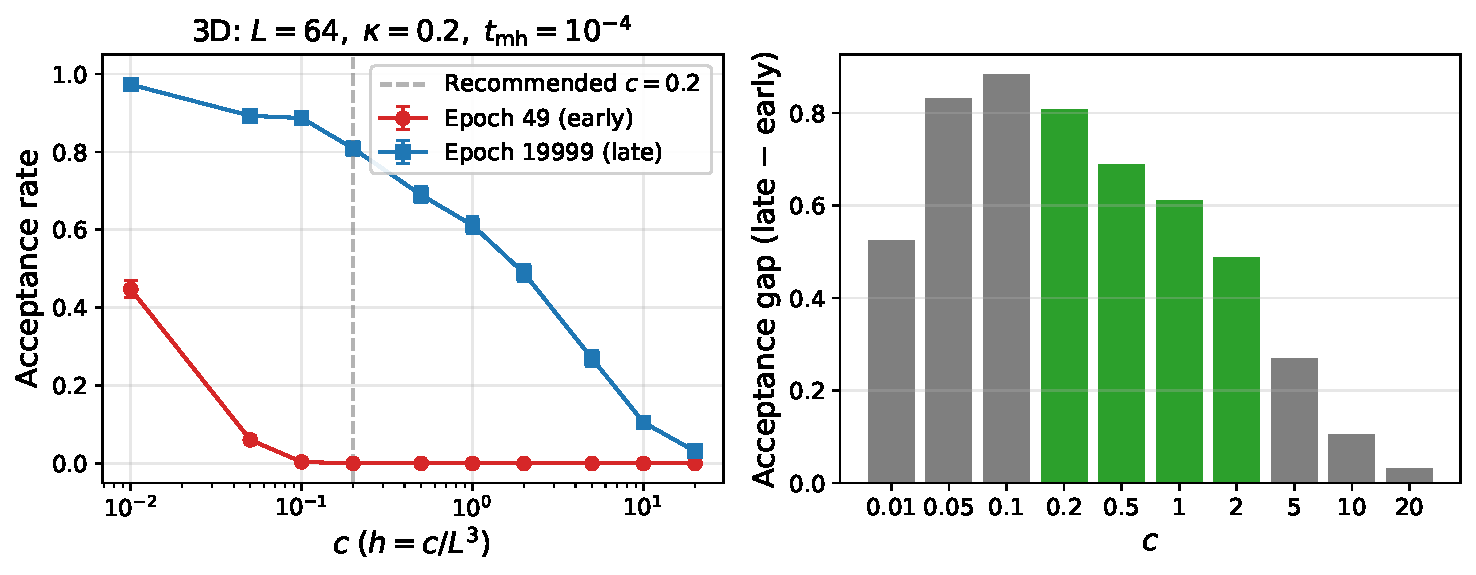
\includegraphics[width=\textwidth]{calibrate_h_3d_L64_k0.2.pdf}
    \end{figure}
    \vspace{-0.3cm}
    {\small $h=c/L^3$: optimal $c=0.2$ (same as 2D!).\\
    Validates $h=c/L^D$ scaling.}
\end{column}
\begin{column}{0.5\textwidth}
    \begin{figure}
        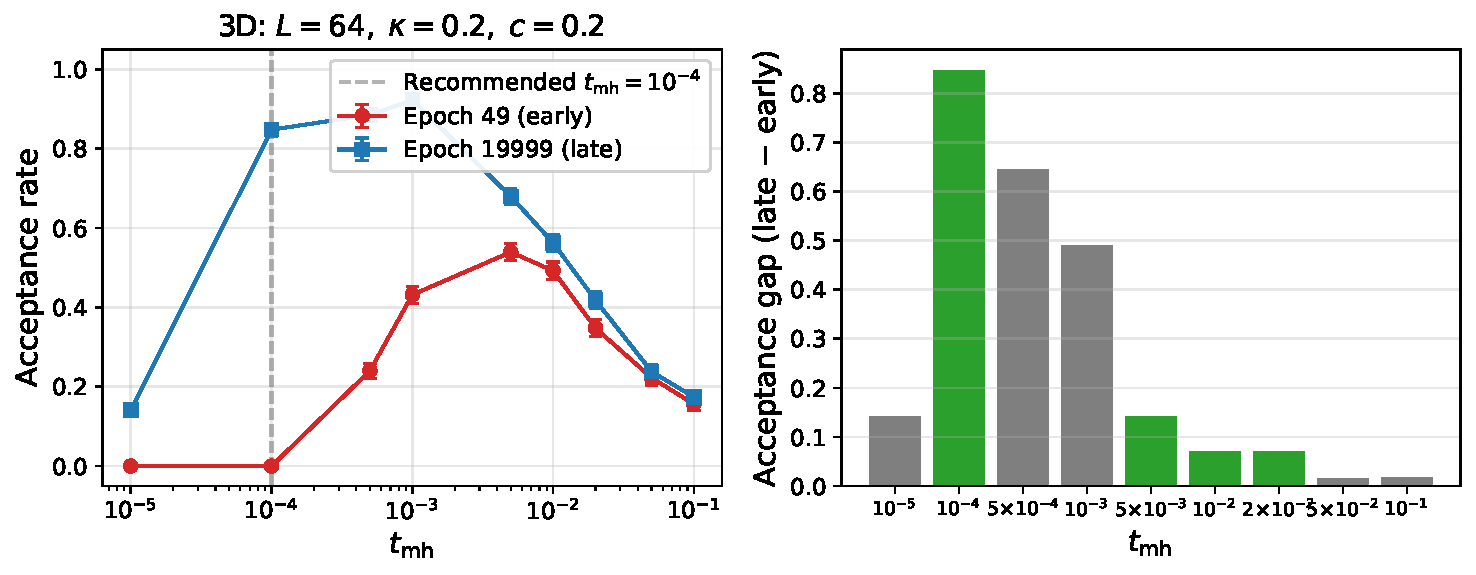
\includegraphics[width=\textwidth]{calibrate_t_mh_3d_L64_k0.2.pdf}
    \end{figure}
    \vspace{-0.3cm}
    {\small $t_\text{mh}=10^{-4}$ optimal (consistent with 2D).}
\end{column}
\end{columns}
\end{frame}

\begin{frame}{3D: Acceptance Rate vs.\ Training Epoch}
\begin{columns}[T]
\begin{column}{0.55\textwidth}
    \begin{figure}
        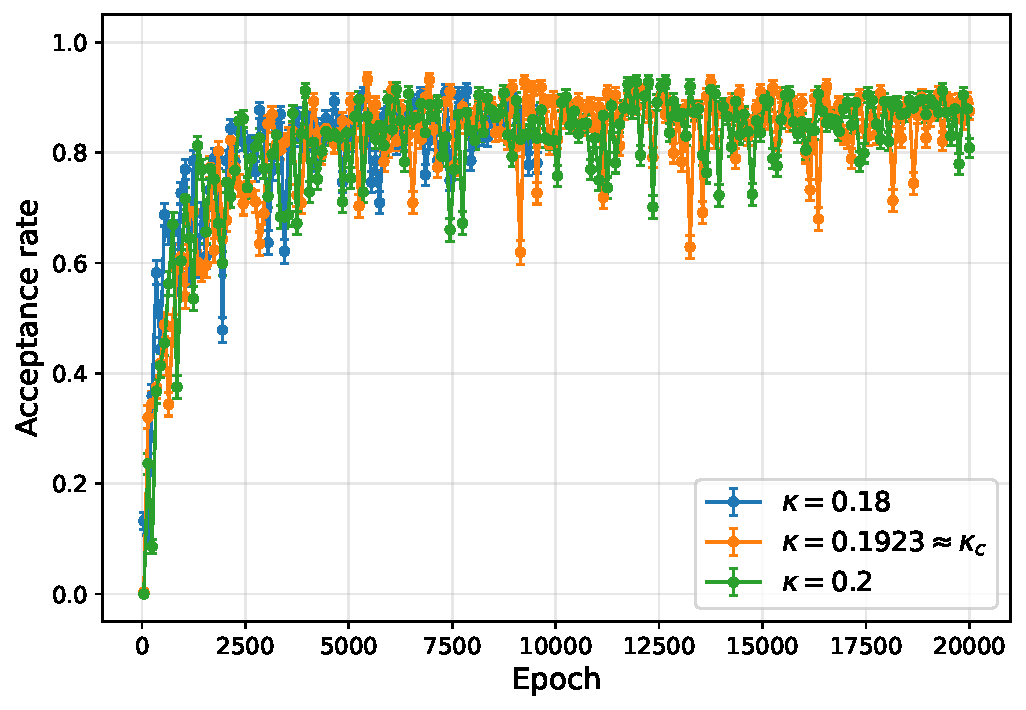
\includegraphics[width=\textwidth]{acceptance_vs_epoch_3d_L64_combined.pdf}
    \end{figure}
\end{column}
\begin{column}{0.45\textwidth}
    \vspace{0.8cm}
    $L=64$, $\lambda=0.9$, $c=0.5$, $h=c/L^3$.
    \vspace{0.3cm}
    \begin{itemize}
        \item Acceptance rate reaches $60$--$90\%$ at late epochs
        \item Comparable to 2D results
        \item Confirms $h=c/L^D$ diagnostic across dimensions
    \end{itemize}
\end{column}
\end{columns}
\end{frame}

\begin{frame}{3D: Direct Score Quality}
\begin{figure}
    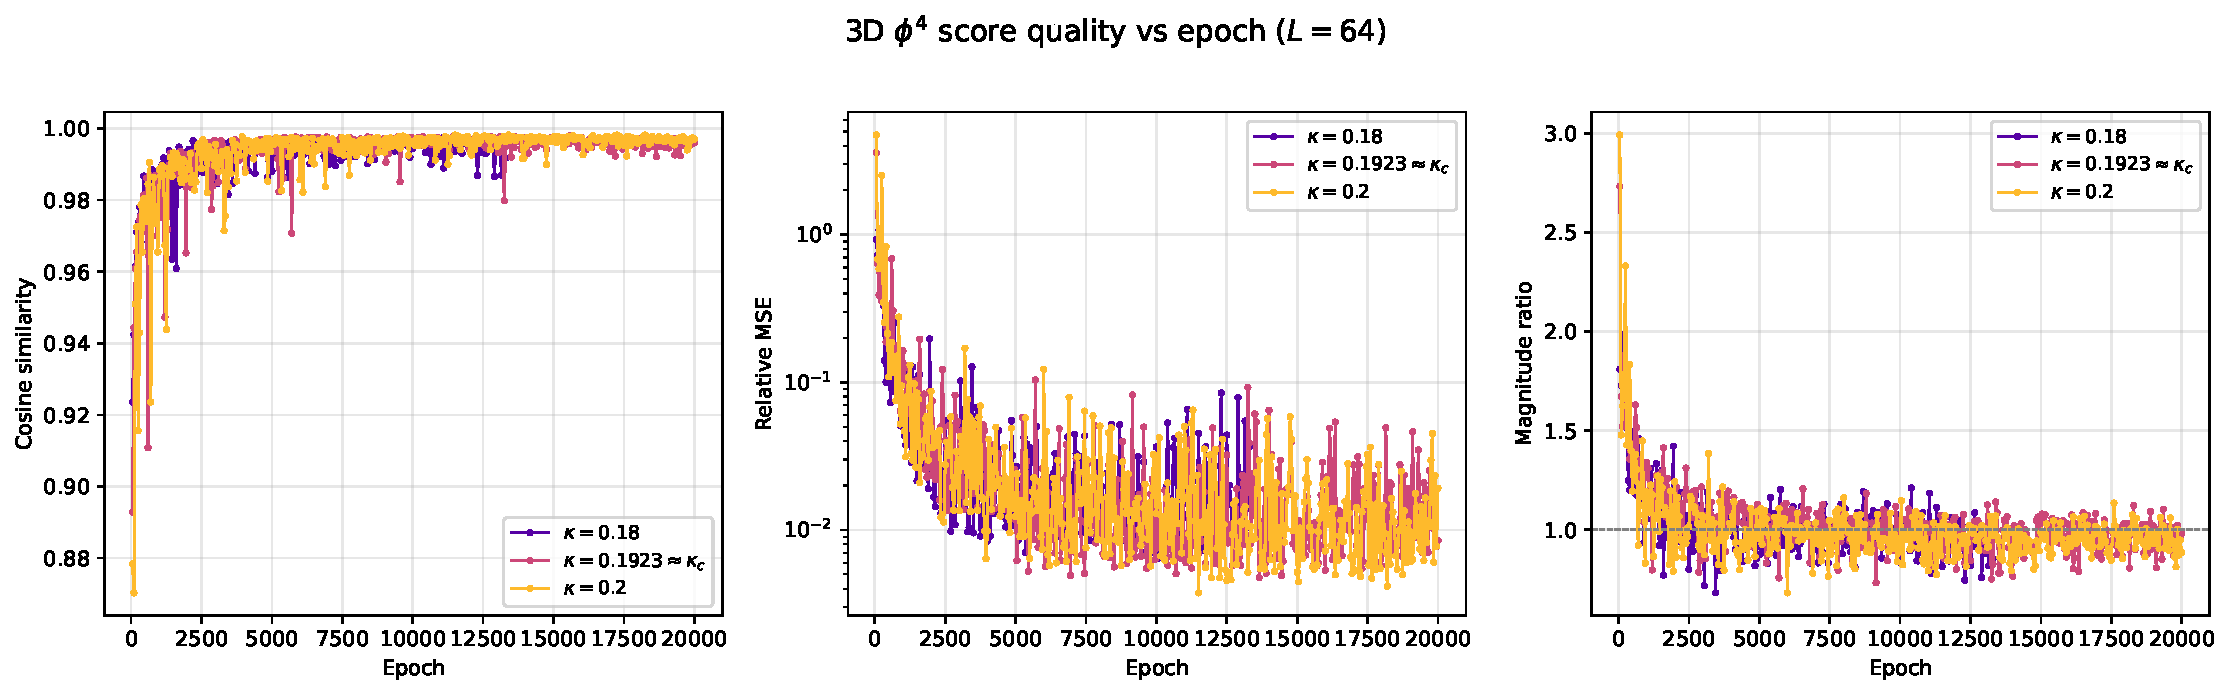
\includegraphics[width=\textwidth]{score_quality_3d_3panel.pdf}
\end{figure}
\vspace{-0.3cm}
$L=64$, $\lambda=0.9$, evaluated at $t_\text{eval}=10^{-4}$ with $N=64$ reference configs:
\begin{itemize}
    \item Cosine similarity: $0.96 \to 0.995$
    \item Relative MSE: drops $>10\times$
    \item Magnitude ratio: $1.4$--$1.5 \to 0.97$--$1.00$ (mirrors 2D trends)
\end{itemize}
\end{frame}

%======================================================================
\section{Summary}
%======================================================================

\begin{frame}{Summary}
\begin{enumerate}
    \item \textbf{Critical points} established via Wolff + FA-HMC:
    \begin{itemize}
        \item 2D: $\kappa_c(\lambda\!=\!0.022) \approx 0.27088$
        \item 3D: $\kappa_c(\lambda\!=\!0.9) \approx 0.19225$
    \end{itemize}

    \vspace{0.3cm}
    \item \textbf{NCSN++ diffusion model} faithfully reproduces $G(p)$ across all phases (symmetric, critical, broken) for both 2D ($L=128$) and 3D ($L=64$)

    \vspace{0.3cm}
    \item \textbf{Diagnostic tools}:
    \begin{itemize}
        \item MALA acceptance rate with $h = c/L^D$ ($c=0.2$, universal)
        \item Direct score quality: cosine similarity $>0.99$, magnitude ratio $\to 1$
        \item Loss decomposition (UV/mid/IR) identifies phase-dependent difficulty
    \end{itemize}

    \vspace{0.3cm}
    \item \textbf{Key design}: circular padding enforces periodic BC on all convolutions
\end{enumerate}
\end{frame}

%======================================================================
\appendix
\section{Backup}
%======================================================================

\begin{frame}{MALA Log-Acceptance Probability}
Substituting the proposal $\psi - \phi - h\,s_\theta(\phi) = \sqrt{2h}\,\eta$:
\begin{align}
    \log\alpha &= \bigl[S(\phi)-S(\psi)\bigr] + \tfrac{1}{2}\|\eta\|^2 \notag\\
    &\quad - \tfrac{1}{4h}\bigl\|\sqrt{2h}\,\eta + h\bigl[s_\theta(\phi)+s_\theta(\psi)\bigr]\bigr\|^2
\end{align}
\begin{itemize}
    \item Single MH step avoids warm-up bias
    \item $h = c/L^D$ rather than MALA-optimal $d^{-1/3}$ due to nearest-neighbour correlations
    \item Gap reverses sign at large $t_\text{mh}$: score evaluates $\nabla\log p_t \neq \nabla\log p_0$
\end{itemize}
\end{frame}

\begin{frame}{2D Acceptance Rate: All Lattice Sizes}
\begin{columns}[T]
\begin{column}{0.5\textwidth}
    {\small \textbf{Early} (epochs 49--249):}
    \vspace{0.1cm}

    {\footnotesize
    \begin{tabular}{cccc}
    \toprule
    $L$ & $\kappa\!=\!0.26$ & $0.2705$ & $0.28$ \\
    \midrule
    8   & $0.152$ & $0.136$ & $0.129$ \\
    16  & $0.082$ & $0.228$ & $0.031$ \\
    32  & $0.207$ & $0.205$ & $0.297$ \\
    64  & $0.288$ & $0.375$ & $0.300$ \\
    128 & $0.336$ & $0.325$ & $0.296$ \\
    \bottomrule
    \end{tabular}
    }
\end{column}
\begin{column}{0.5\textwidth}
    {\small \textbf{Late} (epochs 3999--4999):}
    \vspace{0.1cm}

    {\footnotesize
    \begin{tabular}{cccc}
    \toprule
    $L$ & $\kappa\!=\!0.26$ & $0.2705$ & $0.28$ \\
    \midrule
    8   & $0.635$ & $0.715$ & $0.627$ \\
    16  & $0.683$ & $0.641$ & $0.693$ \\
    32  & $0.680$ & $0.753$ & $0.683$ \\
    64  & $0.827$ & $0.818$ & $0.747$ \\
    128 & $0.790$ & $0.792$ & $0.749$ \\
    \bottomrule
    \end{tabular}
    }
\end{column}
\end{columns}
\vspace{0.4cm}
$c=0.2$, $t_\text{mh}=10^{-4}$, $N=1024$, single MH step.
\end{frame}

\begin{frame}{2D Score Quality: All Lattice Sizes}
\begin{columns}[T]
\begin{column}{0.5\textwidth}
    {\small \textbf{Early} (epochs 49--249):}
    \vspace{0.1cm}

    {\footnotesize
    \begin{tabular}{cccc}
    \toprule
     & \multicolumn{3}{c}{Mag.\ ratio} \\
    \cmidrule(lr){2-4}
    $L$ & $0.26$ & $0.2705$ & $0.28$ \\
    \midrule
    8   & $2.10$ & $2.02$ & $1.94$ \\
    32  & $1.70$ & $1.65$ & $1.57$ \\
    128 & $1.51$ & $1.47$ & $1.46$ \\
    \bottomrule
    \end{tabular}
    }
\end{column}
\begin{column}{0.5\textwidth}
    {\small \textbf{Late} (epochs 3999--4999):}
    \vspace{0.1cm}

    {\footnotesize
    \begin{tabular}{cccc}
    \toprule
     & \multicolumn{3}{c}{Mag.\ ratio} \\
    \cmidrule(lr){2-4}
    $L$ & $0.26$ & $0.2705$ & $0.28$ \\
    \midrule
    8   & $1.28$ & $1.15$ & $1.27$ \\
    32  & $1.05$ & $1.01$ & $0.95$ \\
    128 & $0.91$ & $0.94$ & $0.95$ \\
    \bottomrule
    \end{tabular}
    }
\end{column}
\end{columns}
\vspace{0.4cm}
Cosine similarity $>0.99$ for all $L\geq 32$ at late training.

Magnitude ratio converges to $\sim 1$ for $L\geq 32$.
\end{frame}

\end{document}
